\documentclass[12pt,hyperref=true,mathserif]{beamer}

% Package and Theme
\usepackage{amsmath}
\usepackage{url}
% I suppose listings is no longer needed.
% \usepackage{listings}
\usetheme{AnnArbor}
\graphicspath{{Figure/}{figures/}{figure/}{pictures/}{picture/}{pic/}{pics/}}

% Document Begin
\begin{document}
\title{Revenge of the Nerds}
\author{Yanan Xiao}
\institute[Masdar Institute]{Masdar Institute of Science and
  Technology}
\date[CIS502 Presentation]{Software Engineering Course Presentation}

% Frame Begin
\begin{frame}
\titlepage
\end{frame}

\begin{frame}
  \tableofcontents
\end{frame}

\section{Introduction}


\begin{frame}
% \centering
\begin{center}
``Programming languages have almost caught up with 1958.''
\end{center}
\hfill Paul Graham  
\end{frame}

\begin{frame}
  \frametitle{A Bit of History}
  \begin{columns}
    \begin{column}{0.5\textwidth}
      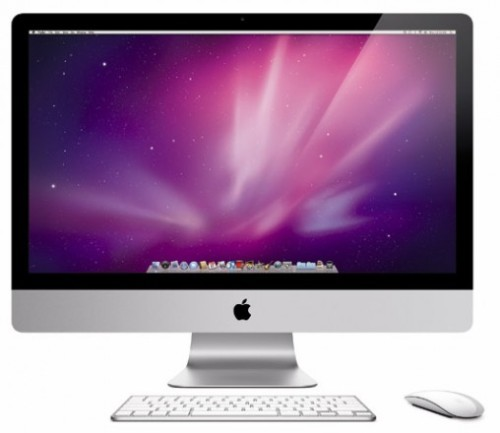
\includegraphics[scale=0.3]{Figure/iMac-500}
    \end{column}
    \begin{column}{0.5\textwidth}
      Question about \emph{computation}.\\[4pt]
      If we had machines that have \textbf{infinite}
      computational power,\\
      what problems would we be able to solve?
    \end{column}
  \end{columns}
  
\end{frame}

\begin{frame}
  Lambda calculus.
  \begin{itemize}
  \item A formal system developed by Alonzo Church.
  \item Essentially a programming language for one of those imaginary
    machines.
  \item Equivalent in power with Turing Machine.
  \end{itemize}
  Lisp.
  \begin{itemize}
  \item Invented by John McCarthy as an implementation of Alonzo's
    lambda calculus, in 1958.
  \item Lisp machine developed by programmers from MIT AI lab, as a
    native hardware implementation.
  \end{itemize}
\end{frame}

\begin{frame}
  \frametitle{Functional Programming ABC}
  \begin{columns}
    \begin{column}{0.5\textwidth}
      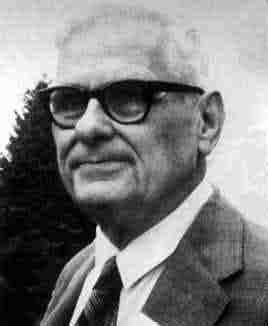
\includegraphics[scale=0.4]{Figure/Alonzo_Church.jpg}\\
      Alonzo Church
    \end{column}
    \begin{column}{0.5\textwidth}
      \begin{itemize}
      \item A practical implementation of Alonzo Church's ideas.
      \item A set of \textbf{ideas}, not a set of strict
        guidelines.
      \item \textbf{A function is a very basic unit in
          functional programming.}
      \end{itemize}
    \end{column}
  \end{columns}
\end{frame}



\section{Functional Programming at a Glimpse}


\begin{frame}
  \frametitle{Functional or Object-Oriented?}
  Objects are little capsules, containing \ldots
  \begin{itemize}
    \item Some internal states.
    \item A collection of method calls.\\[6pt]
  \end{itemize}
  Functional programming tries to \ldots
  \begin{itemize}
    \item Avoid state changes.
    \item Works with data flowing between \textbf{functions}.\\[4pt]
  \end{itemize}
  In this manner, functional programming can be considered the
  opposite of object-oriented programming.
\end{frame}


\begin{frame}
  \frametitle{Theoretical and Practical Advantages}
Functional design may seem like an odd constraint to work
under\footnote{And it is indeed.}. Why should you avoid objects and
side effects? Some sharp benefits are:
\begin{itemize}
  \item Formal provability.\\[4pt]
  \item Modularity.\\[4pt]
  \item Composability.\\[4pt]
  \item Ease of debugging and testing.\\[4pt]
\end{itemize}
\end{frame}

\begin{frame}
  \begin{itemize}
    \item Formal provability. It's easier to construct a
      \textbf{mathematical proof} that a functional program is correct.\\[4pt]
    \item Modularity. It forces you to break apart your problem into
      \textbf{small pieces}.\\[4pt]
    \item Composability. Over time you will form a personal library of
      utilities. It's because of the modularity benefit.\\[4pt]
    \item Ease of debugging and testing. For debugging: functions are
      generally small and clearly specified. For testing: each
      function is a potential subject fir a unit test.
  \end{itemize}
\end{frame}



\section{More Details}


\begin{frame}[fragile,containsverbatim]
  \frametitle{Concurrency}
A functional program is ready for concurrency without any further
modifications.
\begin{block}{Toy Code in Concurrency}
\begin{verbatim}
String s1 = somewhatLongOperation1();
String s2 = somewhatLongOperation2();
String s3 = concatenate(s1, s2);
\end{verbatim}
\end{block}
As shown above, even if your application is inherently single
threaded, the \textbf{compiler}\footnote{The compiler plays a vital
  role.} can still optimize functional programs to run on multiple CPUs.
\end{frame}

% Add some sample code from Erlang when the Internet is back.
\begin{frame}
  \frametitle{Hot Code Deployment}
In a functional program all state is stored on the stack in the
arguments passed to functions. All we'd really have to do is run a
diff between the code in production and the new version, and deploy
the new code.

\end{frame}

\begin{frame}[fragile,containsverbatim,shrink]
  \frametitle{Higher Order Functions}
Functional languages offer a different kind of abstraction tools that
make you forget you've ever \textbf{liked} modifying variables. One such
tool is the capability to work with \textbf{higher order
  functions}.
\begin{block}{Add Function}
\begin{verbatim}
class add_function_t{
    int add(int i, int j) {
        return i + j;
    }
}

add_function_t add = new add_function_t();
\end{verbatim}
\end{block}
In functions we trust.
% Functions that operate on other functions are called higher order
% functions. It's no different from Java classes.
\end{frame}

\begin{frame}[fragile,containsverbatim]
  \frametitle{Currying}
In a functional language one does not need design patterns because the
language is likely so high level, you end up programming in concepts
that eliminate design patterns all together.
\begin{block}{Currying}
\begin{verbatim}
int pow(int i, int j);
int square(int i)
{
    return pow(i, 2);
}
\end{verbatim}
\end{block}
Recall: \textbf{functions} are passed around as arguments.
\end{frame}

\begin{frame}[fragile,containsverbatim]
In functional programming, it looks like this.
\begin{block}{}
\begin{verbatim}
square = int pow(int i, 2);
\end{verbatim}
\end{block}
This will automatically create a function \emph{square} for us with
one argument.
\end{frame}


\begin{frame}
  \frametitle{Lazy Evaluation}
Operations can only be run when another function depends on
them\footnote{Thank you! Compiler.}. Some advantages are \ldots
\begin{itemize}
  \item Optimization. Code can be reasoned about
    mathematically\footnote{Revenge of the nerds!}. 
  \item Abstracting control structures. Seemingly impossible code can
    be implemented.
  \item Infinite data structures. With functional programming, we can
    simply define an infinite list of Fibonacci numbers. 
\end{itemize}
Disadvantage. It's ``lazy''. No strict evaluation can be guaranteed. 
\end{frame}

\begin{frame}[fragile,containsverbatim]
  \frametitle{Continuation}
A ``continuation'' is a parameter we may choose to pass to our
function that specifies where the function should return.
\begin{block}{Continuation}
\begin{verbatim}
int i = add(5, 10);
int j = square(i);
### A continuation approach ###
int j = add(5, 10, square);
\end{verbatim}
\end{block}
At any given point you can ask for a \textbf{current continuation},
which is simply the information on the stack.
\end{frame}


\begin{frame}
  \frametitle{Real World Applications}
The Erlang programming language, developed by Ericsson.
\begin{itemize}
\item originally used in fault-tolerant telecommunications systems.
\item be popular among companies like  T-Mobile, Nortel, Facebook, Electricite de France and WhatsApp.\\[6pt]
\end{itemize}
The Scheme programming language, a dialect of lisp, is taught at a
graduate level course\footnote{\url{http://mitpress.mit.edu/sicp/}} in MIT.
\end{frame}


\section{The Dream Language}


\begin{frame}
% \bibliographystyle{plain}
% \bibliography{Reference}
The dream language is clean and terse. It has an interactive top level
that starts up fast. You can write programs to solve common problems
with very little code. Nearly all the code in any program you write is
code that's specific to your application. Everything else has been
done for you.\\
% \begin{itemize}
%   \item Clean and terse.
%   \item Has an interactive top level that stars up fast.
%   \item 
% \end{itemize}
\hfill Excerpt from ``Hackers and Painters''
\end{frame}







\end{document}


% Someone is like you.
